In this chapter, our framework will be evaluated using a variation of the Goal-QuestionMetric (GQM) technique \cite{van2002goal}. The GQM plan has been slightly modified by the addition of a new column with the results. The questions pertinent to evaluating our strategy and its outcomes are separated into two primary sections: the first related to the algorithm utilized in the pattern analysis process itself, and the other about the method's overall efficacy. Table \ref{tab:gqm_plan} details the study questions.

\begin{table}[!h]
    \centering
    \begin{tabular}{ccl}
    \hline
    \multicolumn{3}{|c|}{\textbf{Goal 1}: Property Violation Identification process}                                                                                                                            \\ \hline
    \multicolumn{1}{|c|}{Question}                                                                                    & \multicolumn{1}{c|}{Metric}                     & \multicolumn{1}{l|}{Results} \\ \hline
    \multicolumn{1}{|c|}{\makecell{How well does our model \\ generalizes to unseen data?}}                                         & \multicolumn{1}{c|}{\makecell{Precision and \\Recall Rates}} & \multicolumn{1}{c|}{\makecell{Precision: 1.0 \\ Recall: 0.9958}}        \\ \hline
                                                                                                                      &                                                 &                              \\ \hline
    \multicolumn{3}{|c|}{\textbf{Goal 2}: Method's contribuition}                                                                                                                                               \\ \hline
    \multicolumn{1}{|c|}{Question}                                                                                    & \multicolumn{1}{c|}{Metric}                     & \multicolumn{1}{l|}{Results} \\ \hline
    \multicolumn{1}{|c|}{\makecell{How effective is our approach \\ in the discovery of patterns \\in property violation scenarios?}} & \multicolumn{1}{l|}{\makecell{Number of \\patterns found}}   & \multicolumn{1}{c|}{}        \\ \hline
    \end{tabular}
    \caption{GQM Plan}
    \label{tab:gqm_plan}
\end{table}

\section{Experimental Setup}

The evaluation of our proposed solution will rely on a implementation of the Body Sensor Network from Section \ref{BSN}. Our version of this CPS includes a Central Node and five sensors: an oximeter, a thermometer, a heart rate monitor, and an APBD and APBS blood pressure sensors. The patient's readings are assessed within each sensor node, where the health risk percentage of the monitored vital sign is calculated. Subsequently, the risk percentage is relayed to the Central Node, which, in turn, is in charge of collecting and fusing the data from the sensors, assessing the patient's overall risk, and indicating an emergency if one is discovered.

\subsection{Prototype Implementation}

The first part of our technique requires the implementation of a CPS prototype. This is done to anticipate problems that may occur during runtime by modeling and simulating both the system's software components and physical processes. Despite the fact that there are several state-of-the-art approaches for designing such models \cite{baras2019formal} \cite{deng2019modeling} \cite{bouskela2022formal}, and since the focus of this work is to elaborate on the property violation patterns using the NSA, a simpler framewrok for the simulation was selected. The Modelica language \cite{Modelica}, hence, will be used as the main tool in this process. This language is powerfull enough to represent the acausal continuous-time physical processes of the CPS through equations. It also comprises several built-in libraries for the modeling of circuits, batteries, fluids, noise, equipment deterioration and so on. At the same time, software components can also be described by defining algorithms and functions that account for the behavior of such modules. The graphical aid is achieved by the OpenModelica \cite{OpenModelica} modeling tool, in which the components and their interactions can be visually modeled as blocks and connectors.

\begin{figure}[!h]
	\centering
	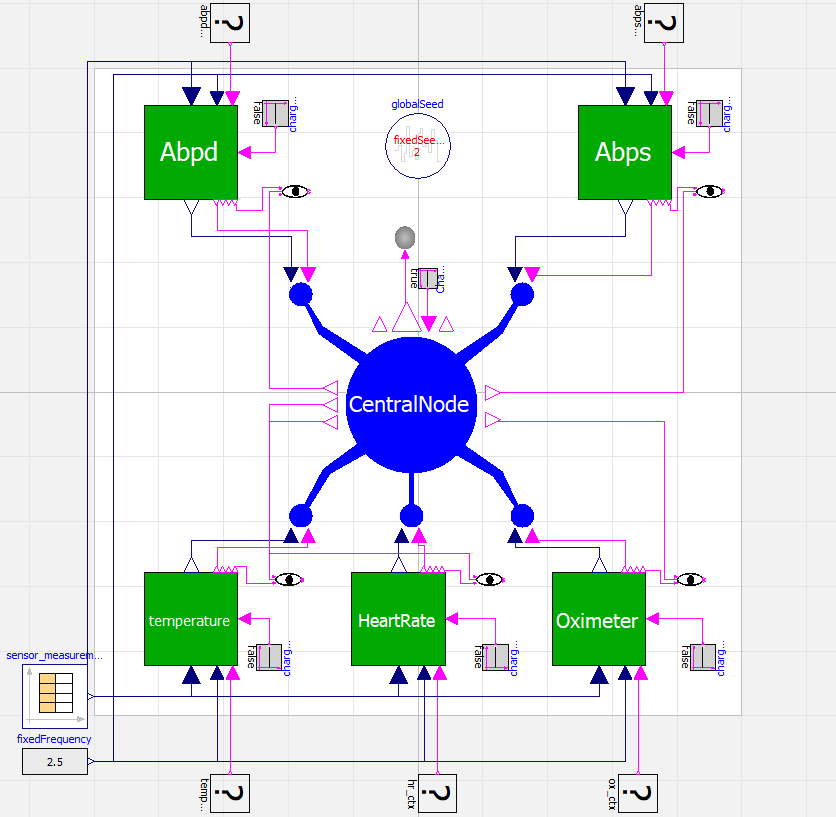
\includegraphics[width=0.7\textwidth, keepaspectratio]{img/BSN_prototype_Modelica.png}
	\caption{BSN Prototype Implemented in OpenModelica}
	\label{fig:BsnProt}
\end{figure}

Figure \ref{fig:BsnProt} depicts the prototype that was implemented in OpenModelica, using the Modelica language. The green blocks account for the sensors, while the blue illustrates the Central Node. In the left lower side, a parameter defines a fixed frequency for data collection that is utilized by every sensor, and above it there is a reference for an external csv file that contains the measurements of the sensors at every second. Around the system, there are some blocks with question marks whose function is to generate random binary numbers to indicate whether the sensor was active. The goal of these blocks is to simulate cases when the sensor stopped responding, or was to far away to transmit reliable data, or had some malfunctioning of sorts that may account for faults in runtime. Next to the sensors there are some gray boxes that are used to indicate when the sensor is plugged into the outled. Besides that, there are also small rounded blocks that represent the observers, that are modeled to monitor the system properties.

\begin{figure}[!h]
	\centering
	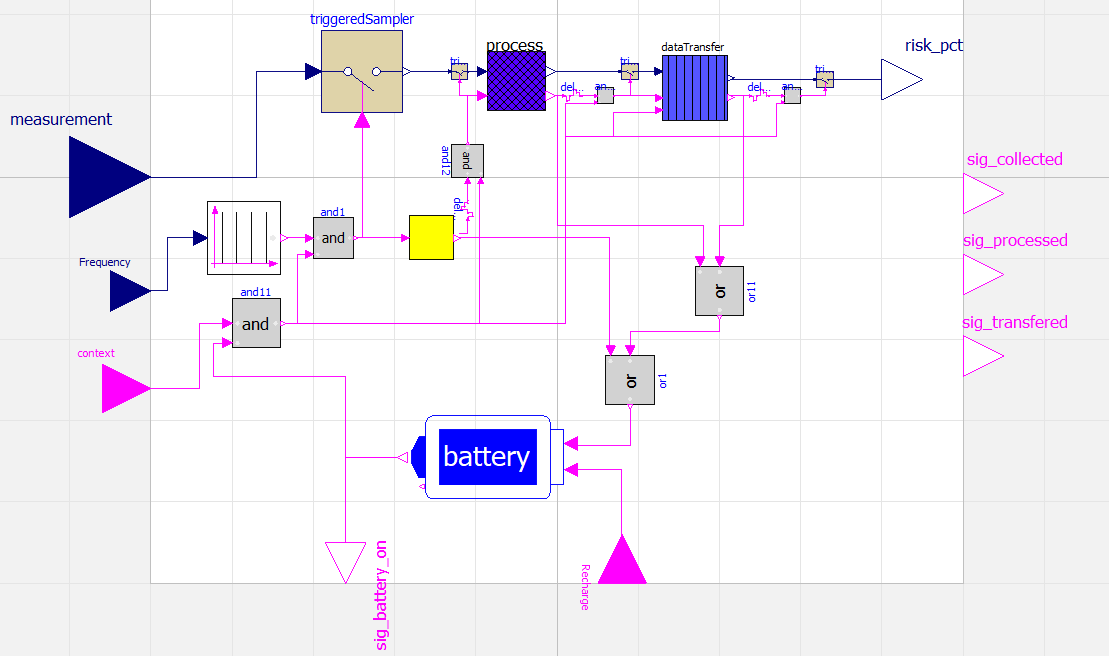
\includegraphics[width=0.7\textwidth, keepaspectratio]{img/sensor_modelica.png}
	\caption{The model of a sensor implemented in OpenModelica}
	\label{fig:sensorProt}
\end{figure}

By going one step deeper into the model, it is possible to describe how the inner workings of the sensors and the Central Node were implemented. One of the advantages of the Modelica language is its object-oriented character that allows for the reuse of modules throughout the simulation. The sensor described in Figure \ref{fig:sensorProt} is a good example of this aspect, since the same block is used to model all five sensors. The physical components represented here comprise: a mechanism for sampling a measurement based on a triggered signal, a set of bitwise operators that are often used in microcontroller programming, and a battery. This battery was modeled based on a built-in Modelica library that allows for the modeling of electric circuits, and is composed of a set of switches, a memory cell, and a signal current converter that receives signals from the sensor whenever some process occur to decrease the charge of the memory cell. The magnitude of the charge decrease is multiplied by a randomly generated real number in a way to simulate the decrease that would happen in a real environment. In the meanwhile, software components of the sensor are also modeled, like the Process block, which recieves a real valued sensor measurement as an input and relies on an algorithm for determining the health risk percentage of the patient.

\begin{figure}[!h]
	\centering
	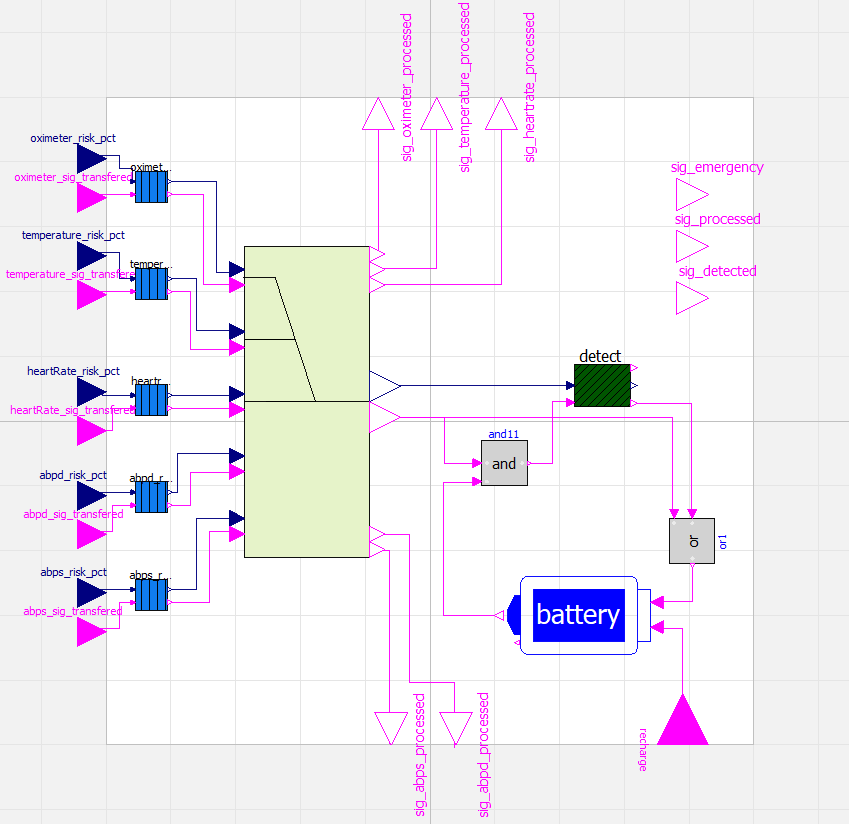
\includegraphics[width=0.7\textwidth, keepaspectratio]{img/central_node_modelica.png}
	\caption{The model of the Central Node implemented in OpenModelica}
	\label{fig:centralNodeProt}
\end{figure}

The Central Node, illustrated in Figure \ref{fig:centralNodeProt}, was implemented in a similar fashion. It also makes use of bitwise operations for handling the signals sent, and of an instance of the same battery model as the one found in the sensors. The software components encapsulate functions that fuse the data from the sensors and compute the overall health risk of the patient.

Both the sensors and the Central Node are instrumented through a set of signals that are sent each time a process or a specfic behavior occur, like when the data is collected or transfered for instance. These signals are used by the observers to monitor the properties of interest, and will be used later for the characterization of a execution segment, during the pattern analysis phase. Observers can be easily modeled in Modelica via a built-in library developed for the desing of state graphs. Both the states of the automata and its transitions are described as blocks, with the difference being that the transitions receive signals as input to indicate the passing through the states. Figure \ref{fig:obsProt} illustrates the observer implementation in Modelica utilized in throughout the evaluation.

\begin{figure}[!h]
	\centering
	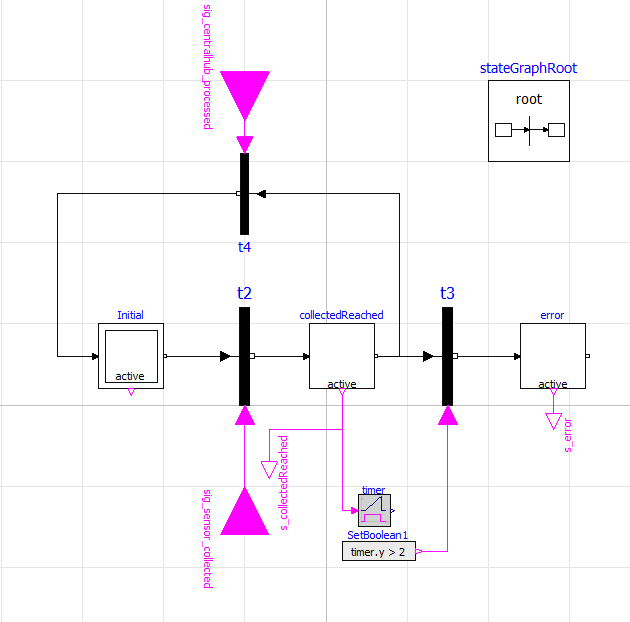
\includegraphics[width=0.5\textwidth, keepaspectratio]{img/obs_modelica.png}
	\caption{The model of the Observer implemented in OpenModelica}
	\label{fig:obsProt}
\end{figure}

\subsection{Prototype Simulation}

With the prototype of the BSN in place, several simulations were executed with varying configurations, patient profiles and environment variables so that the complexities of runtime could be assessed earlier. 

As noted in the preceding section, one of the simulation's inputs is a csv file holding the sensors' readings at each second. The patient profile given by these files is constructed using a randomized approach in the Python language in order to be as neutral as feasible. Three functions for generating random points within a range were created: one for indicating a rising tendency, another for indicating a decreasing tendency, and a third for keeping the data steady. Initially, a random point is created within the sensor's range of data. Then, one of the three functions and a second value that accounts for the "destination" are randomly picked. The function is then run for the generation of data points starting from the initial value and ending in the destination value, with the selected tendency. For large datasets, the process can be repeated with the destination value becoming the initial value of the new cycle. For example, suppose we are generating the data for the thermometer. The initial value is 36.5C, the destination value generated is 38C and the selected function is the rising tendency. Then a set of datapoints will be randomly genereated in a way that it starts from the initial value and rises until reaching 38C. This process was performed for each of the five sensors and repeated until the desired data set size.

After the creation of the dataset, the simulation was run. Even though OpenModelica makes it realy easy to perform simulations, it does not scale weell, since the csv fileas and the system configurations must be set manually at each run. To address this problem, a python library named OMPython was used \cite{OMPython}. It is a Python-based interactive session handler for Modelica scripting that is free, open source, and extremely portable. It was utilized to programatically load the modules, alter the parameters and configurations and run the simulation.

To account for as much variability as possible, 1,000 patient profiles were randomly generated and, the same amount of simulations were performed. The operation dataset of each run was extracted and saved as csv files. The simulation was processed in an Intel(R) Core(TM) i5-10210U, 2.10 GHz, 16GB.

\section{Goal 1: Property Violation Identification process}

\section{Goal 2: Method's contribuition}

\section{Discussion}

\section{Threats to validity}